\documentclass[12pt,letterpaper]{article}

%Packages
% \usepackage{textcomp}
% \usepackage{latexsym}
% \usepackage{url}
% \usepackage{amssymb}
% \usepackage{amsmath}
% \usepackage{mathtools}
% \usepackage{bm}
% \usepackage{array}
% \usepackage[version=3]{mhchem}
% \usepackage{ifthen}
% \usepackage{amsthm}
% \usepackage{amstext}
% \usepackage{enumerate}
% \usepackage{dcolumn}

\usepackage{epsfig}
\usepackage{graphicx}
\usepackage{caption}
\usepackage{hyperref}
\usepackage{lineno}
\usepackage{pdflscape}
\usepackage{mathtools}
\usepackage[osf]{mathpazo}
\usepackage{fullpage}
\usepackage{float}
\usepackage{xr} %linking to supplementaries
\usepackage{xcolor}
\externaldocument{supplementaries}

\pagenumbering{arabic}


%---------------------------------------------
%
%       START
%
%---------------------------------------------

\begin{document}
\noindent \today
\bigskip

\noindent Dear editor,
\bigskip

We are grateful for the detailed and useful comments from all four reviewers. We have taken all their suggestions on board, integrated changes associated with the suggestion into the manuscript and responded to them in detail below. For clarity we have displayed \textcolor{blue}{the reviewers’ comments in blue} and our own responses in black.

We have revised  the manuscript taking advantage of the extra space and number of figures allowed for Science Advances. Briefly, the major changes are:

\begin{itemize}
    \item We now clearly distinguish the two types of elaboration and innovation: $elaboration_{species}$ and $innovation_{species}$ that focuses on the macro-evolutionary scale and $elaboration_{clades}$ and $innovation_{clades}$ that focuses on the mega-evolutionary scale;
    \item For the analyses on elaboration and innovation at the macro scale ($elaboration_{species}$ and $innovation_{species}$), we now only focus on the projection of species onto their order’s major axes;
    \item We added two new figures and a table in the main text: the cheat sheet figure (previously in the supplementaries, now in the introduction), the correlation figure and a table from the new PGLS results; 
    \item We have added several new analyses to the supplementary materials including: correlations between elaboration/innovation, elaboration and innovation through time and random skewers analysis;
    \item We have linked our metrics definitions to previous work in the supplementary materials;
    \item We have made the vocabulary more consistent throughout the manuscript;
    \item We fully rewrote the introduction and most of the results/discussion section.
\end{itemize}

We fully describe each change below.
\bigskip
Best regards,
\bigskip
Thomas Guillerme, on behalf of all co-authors.

\section*{\textcolor{blue}{Reviewer 1}}

\textcolor{blue}{This study is an important contribution to the field of phenotypic macroevolution, and I strongly recommend its publication. The conceptualisation is very interesting, and I am aware that it represents the culmination of many years of research by the group/s involved, whose contributions I have seen several times along the years in several conferences. The authors devise a smart new method to evaluate the contributions of elaboration (i.e., evolutionary change along the major axis of variation of a clade) against innovation (i.e., evolutionary change away from this major axis).}

\textcolor{blue}{However, I have one major problem with the interpretation of the results. I will use an example to illustrate my point:}

\textcolor{blue}{Lines 108-110 go: ‘For example, compared to the global phylogenetic major axis of phenotypic variation, the Trochilidae (hummingbirds) in the order Apodiformes, have long narrow beaks and display high levels of elaboration and low innovation’.}

\textcolor{blue}{One could argue that the beak shape of hummingbirds represents one of the most exceptional cases of niche expansion and beak shape innovation in birds (Cooney, Bright et al., 2017, Nature). We know from the fossil record that hummingbirds likely evolved from broad-billed ancestors (i.e., stem trochilid Parargornis) so in reality, this comparison might not faithfully represent the actual evolutionary process undergone by crown group hummingbirds (high innovation as it departs from the main axis of evolutionary variation within strisoreans). Therefore, I am not sure I see what species values of ‘innovation’ and ‘elaboration’ in this context (i.e., compared to the global axis of whole-Neornithes variation) are telling us about the actual underlying innovation and elaboration as real evolutionary forces.}

\textcolor{blue}{I think the appropriate comparison for species values of innovation and elaboration might be with the main axes of variation of the immediately superior phylogenetic scale (order level in this case). Comparisons of species level values derived from the main axis of variation at the level of whole Neornithes might reflect global constraints in beak shape. For instance, coming back to the hummingbirds, there is some evidence that the divergence in cranial shape between hummingbirds and the remaining strisoreans might be related with a reversal to an ontogenetic trajectory that is pervasive among non- strisorean birds (Navalon et al., 2021, Proc. B). The similarities in beak shape between hummingbird species and the main axis of beak shape variation (long and slender to short and stout) in this study might reflect general constraints in beak shape variation rather than anything else. I think therefore conflating species level data from the whole-Neornithes axis with species level data from the order or parvorder axes might be confounding two kinds of data, different in nature, although, admittedly, it is intriguing that the same pattern (elaboration higher than innovation) holds at all the different phylogenetic levels.}

\textcolor{blue}{I suggest therefore keeping only the species level values as compared with the main axis of variation at the order/parvorder level as indicating ‘true’ innovation and elaboration. The comparisons of the main axis between different clades, in my opinion, indicate deep divergences in the main axes of beak shape variation. So I suggest keeping those too. Then either ditching the comparisons of species level dispersion values with whole- Neornithes or reinterpreting them.}

\textcolor{blue}{As a result, I am not entirely convinced with the authors conclusion that accumulated gradual elaboration creates deep divergences among main axes of variation in clades. I might be wrong, but my reading of the presented data is that:
\begin{enumerate}
\item Deep divergences among clades create different patterns of beak shape variation in different orders.
\item Species level beak shape variation within clades is characterised by more elaboration than innovation – evolution along lines of least resistance.
\item Species level variation as compared with the main axis of beak shape variation in whole Neornithes indicates that beak shapes are affected by whole-clade constraints – possibly of developmental nature. Calling this innovation and elaboration and equating it to the concepts in bullet point 2 is confusing in my opinion because it is several levels detached from the actual evolutionary process creating ‘elaboration’ or ‘innovation’.
\end{enumerate}
I reckon my interpretation is aligned with what earlier work by the authors (Cooney, Bright et al., 2017 and more by other authors!) suggest and adds to the discussion by showing the very interesting result that evolutionary variation in beak shape is largely constrained at several levels. But I don’t think it really contributes to ascertaining why deep divergences among clades occur unless further analyses can be carried out.}

We are grateful to the reviewer for pointing out this concern so clearly. We have now clarified what we mean by innovation and elaboration throughout the manuscript. We now consider the following:
\begin{itemize}
    \item Elaboration and innovation at the macroevolutionary scale for each species ($elaboration_{species}$ and $innovation_{species}$) as the projection/rejection of individual species on their order’s major axis of trait variance-covariance. We have moved the projections/rejection of species onto higher taxonomic levels (super-orders and the whole phylogeny) into the supplementary materials.
    \item Elaboration and innovation at the megaevolutionary scale (sensu Simpson 1944, 1953) $elaboration_{clade}$ and $innovation_{clade}$) as the projection/rejection of entire clades (orders or super-orders) onto their higher clades (super-order or the whole phylogeny).
\end{itemize}
We have reframed the whole manuscript and analyses with this in mind and have completely rewritten the introduction. Note that our previous version of the manuscript was a submission to Science and was directly transferred to Science Advances. We have now fully taken advantage of the extra space available which hopefully increases the clarity of the manuscript. This re-framing should remove the issues raised by the reviewer regarding the interpretations of our results.

We now also directly refer to the example suggested by this reviewers on lines 73-77:%@L_strisores_example:

\noindent\textit{For example, a major shift in beak shape arises in the early divergence of Strisores separating hummingbirds (Trochilidae) from swifts (Apodidae), perhaps marking changes in ontogenetic trajectories \cite{navalon2021} as hummingbirds diverged from broad billed ancestors (e.g. the Eocene stem Trochilidae fossils \textit{Parargornis messelensis} and \textit{Eocypselus rowei} \cite{mayr2003new, ksepka2013fossil}).} %@L_strisores_example


\textbf{\textcolor{blue}{More detailed comments:}}

\textcolor{blue}{I think Figure S5 – or a simplified version of it - should be Figure 1 in the main text to guide the readers through the methods and the theoretical framework used in the study. This will be beneficial too for the published paper to be noticed by the community – which I think it might be desirable because it is a very interesting contribution.}

Thanks for the suggestion. We have now reworked Figure S5 and use it as a “cheat sheet” in the introduction to guide the reader through the results of the original figures 1 and 2 (now figures 2 and 4).

\begin{figure}[!htbp]
\centering
   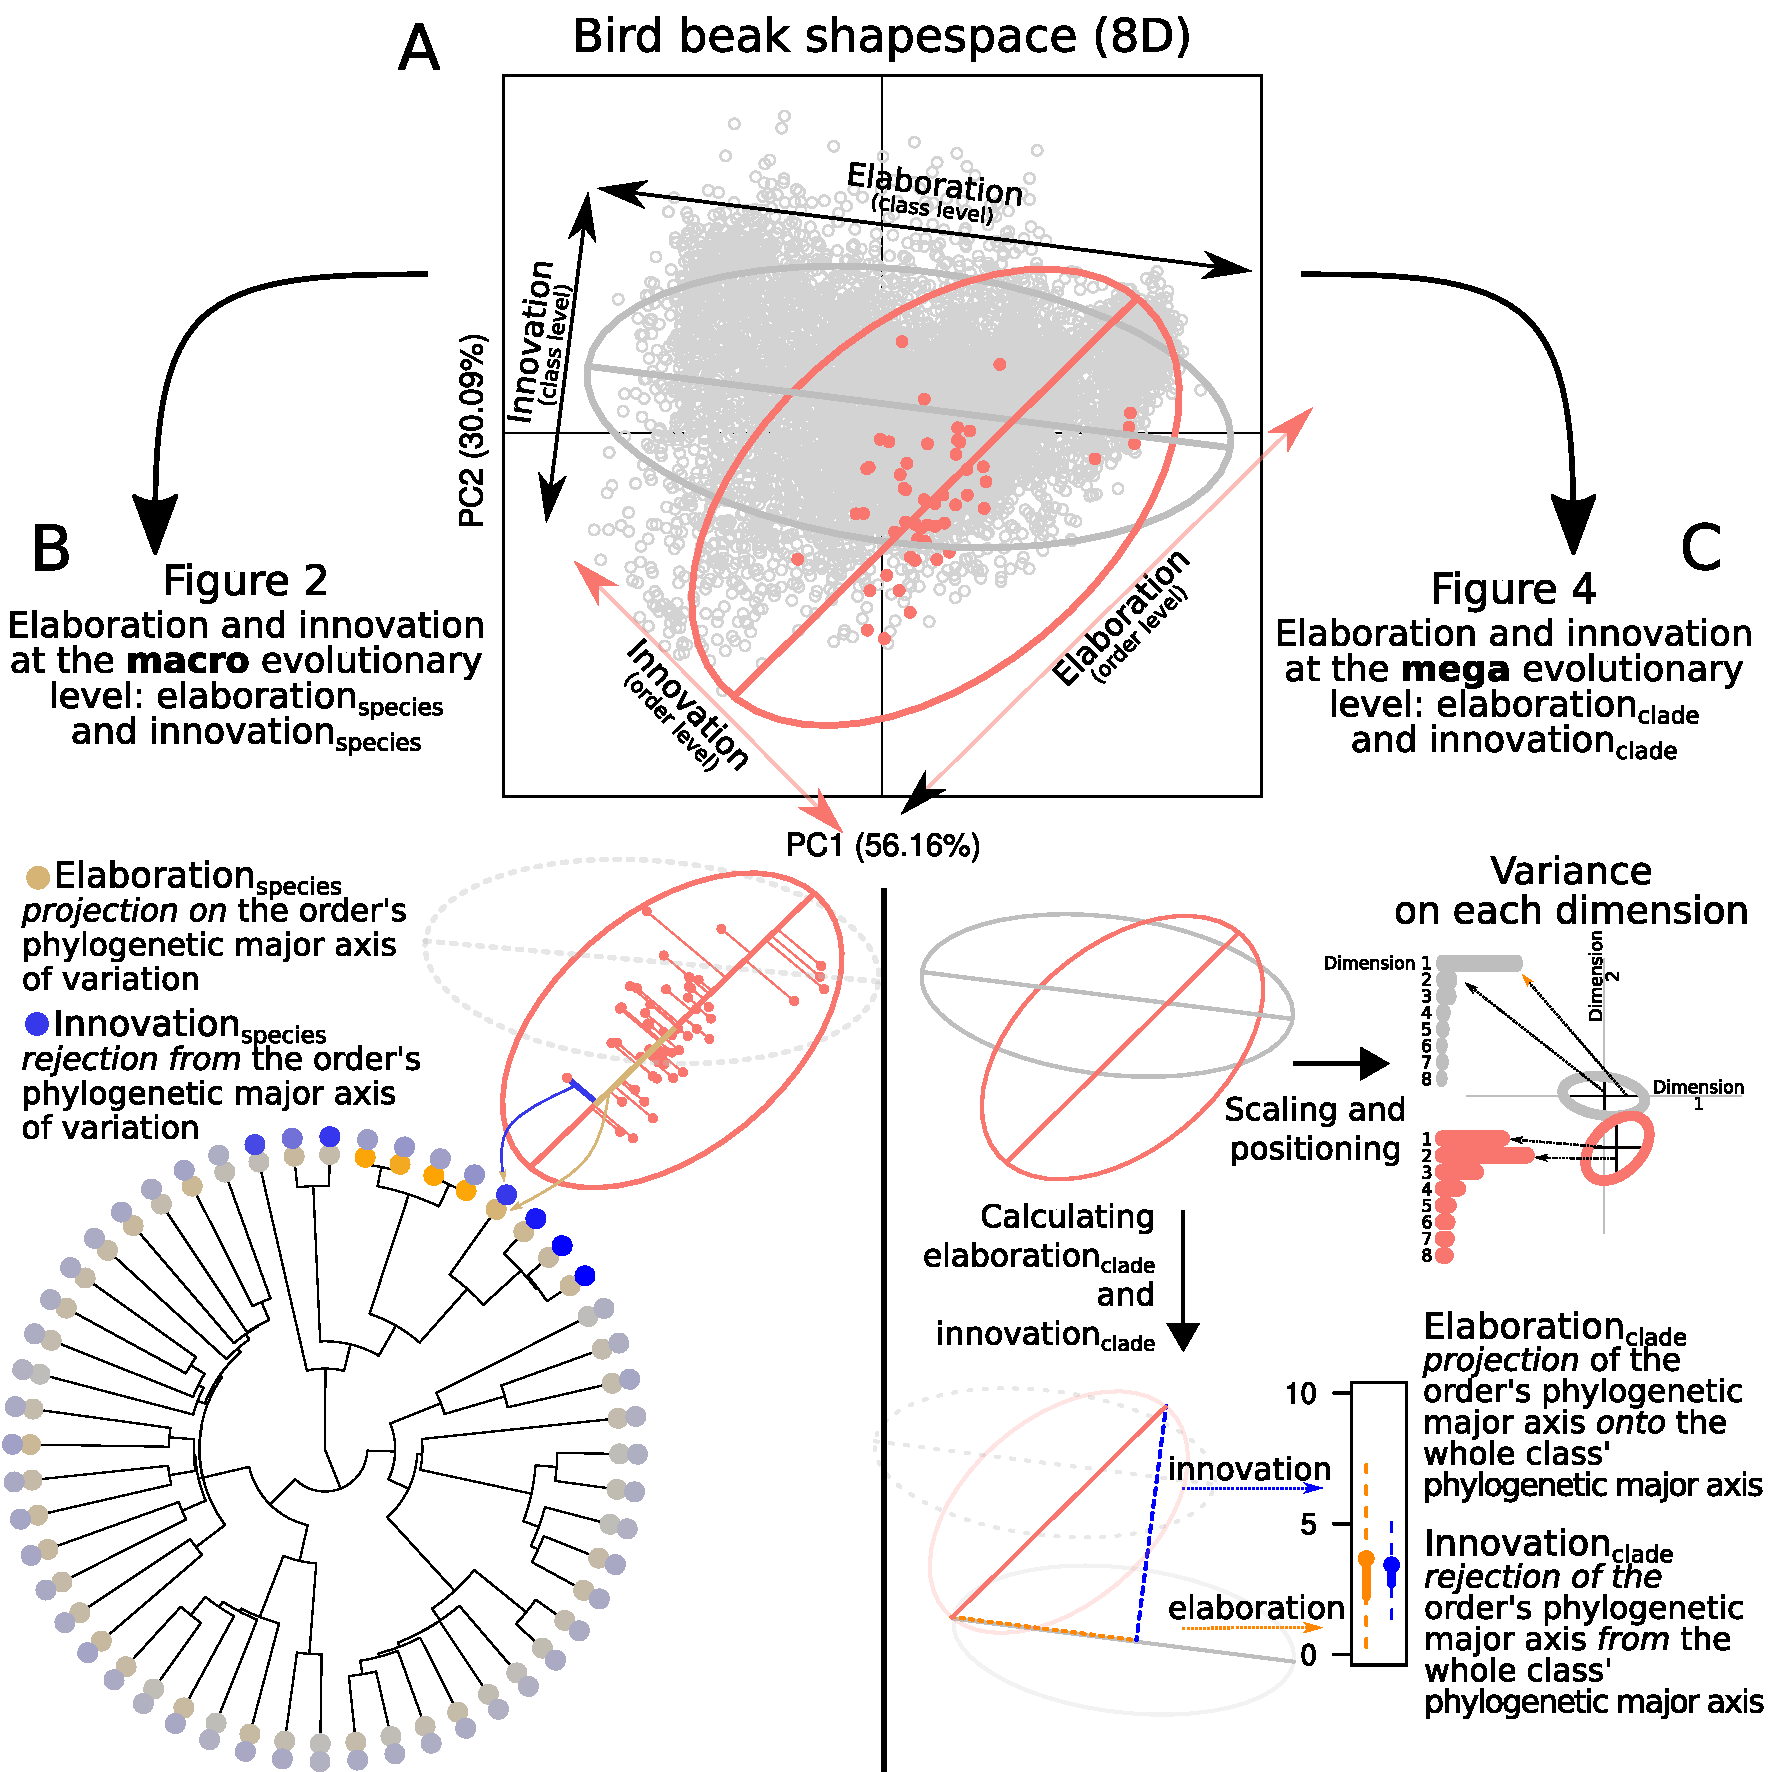
\includegraphics[width=0.6\textwidth]{Figures/cheat_sheet.pdf}
\caption{\scriptsize{Relationships between key figures in the main text.
A) represents the two first principal components (PCs) of the eight dimensional trait space with all bird beak shapes represented as gray circles and the Tinamiformes as red circles.
The gray ellipse represents the overall phylogenetic major axis of beak variation in birds.
Species aligned or away from this axis are respectively elaborators or innovators relative to the class Aves.
The red ellipse and axis represents the phylogenetic major axis of beak variation in Tinamiformes only.
Species aligned or away from this axis are respectively elaborators and innovators relative to the Tinamiformes order.
B) In Figure 2, we measured elaboration and innovation at the macroevolutionary scale , i.e. the position of each species in terms of $elaboration_{species}$ and $innovation_{species}$ relative to their order's phylogenetic major axis of beak variation.
A species $elaboration_{species}$ score is the species projection onto their order's phylogenetic major axis of beak variation(i. e. their position on that axis) whereas their $innovation_{species}$ score is their rejection from it (i.e. their distance away from that axis).
The colours on the tips of the phylogeny correspond to the median $elaboration_{species}$ (orange gradient) and $innovation_{species}$ (blue gradient).
C) Figure 4, we measured elaboration and innovation at the megaevolutionary scale, i.e. $elaboration_{clade}$ and $innovation_{clade}$.
The ellipses are scaled and centered and represent the clade's phylogenetic major axis of beak variation relative to the overall phylogenetic major axis of beak variation with the relative length of the ellipse on each dimension represented on the barplots as variance on each dimension.
A clade's $elaboration_{clade}$ and $innovation_{clade}$ scores are measured by projecting the clade's phylogenetic major axis of beak variation onto the overall phylogenetic major axis of beak variation and measuring the projection (elaboration) and rejection (innovation) from this axis as described above.
The distribution elaboration and innovation scores are taken from the projection of the 4000 pairs of evolutionary rate matrices with each pair being the focal level, e.g. order,and the parent level, e.g. the whole bird phylogeny.}}
\label{Fig:cheatsheet}
\end{figure}

\newpage

\textcolor{blue}{The abstract could benefit from briefly stating (e.g., a parenthesis) what innovation and elaboration are in this context. Similarly, the introduction would benefit from defining very clearly what is meant by micro- macro- and mega-evolution. I guess mega- in this context refers to divergence among major avian clades (order level or similar). Also bear in mind microevolution is within species so it is of limited utility here.}

We have now completely rewritten the abstract and introduction, ensuring we clearly introduce the concepts of innovation and elaboration, and mega-, macro- and micro- evolution. We defined the mega-, macro- and micro- evolutionary scales as the scales focusing respectively on the clades, species and individuals. We also link these concepts to the literature more thoroughly. Note that our previous version was a direct transfer from a journal with a more limited page count, but having more space to explain our approach has improved the manuscript substantially (lines 5-16):

\noindent\textit{Widely documented, megaevolutionary jumps in phenotypic diversity continue to perplex researchers because it remains unclear whether these dramatic changes can emerge from microevolutionary processes.
Here we tackle this question using new approaches for modeling multivariate traits %@L_multi_traits
 to evaluate the magnitude and distribution of elaboration and innovation in the evolution of bird beaks.
We find that elaboration, evolution along the major axis of phenotypic change, is common at both macro- and megaevolutionary scales whereas innovation, evolution away from the major axis of phenotypic change, is more prominent at megaevolutionary scales.
Indeed, the major axis of phenotypic change among species beak shapes at megaevolutionary scales is an emergent property of innovation across clades.
Our analyses suggest that the reorientation of phenotypes via innovation is a ubiquitous route for divergence that can arise through gradual change alone, opening up new avenues for evolution to explore.}

\textcolor{blue}{Lines 104-105: ‘We find no consistent evidence that innovation is either positively correlated, or trades-off, with elaboration’. Have you formally tested this? Maybe it would be good to show a dot plot of this for species values.}

We have now added a new analysis to the supplementary materials where we show the correlation between $innovation_{species}$ and $elaboration_{species}$ and we link to this figure in the main text (Figure 3). We find some variability in this relationship depending whether innovation and elaboration are calculated from comparisons to orders, suborders, or the whole tree. At the order level (our main focus in the new version of the manuscript) we find that positive correlations are common and negative correlations (trade-offs) are absent.


\begin{figure}[!htbp]
\centering
   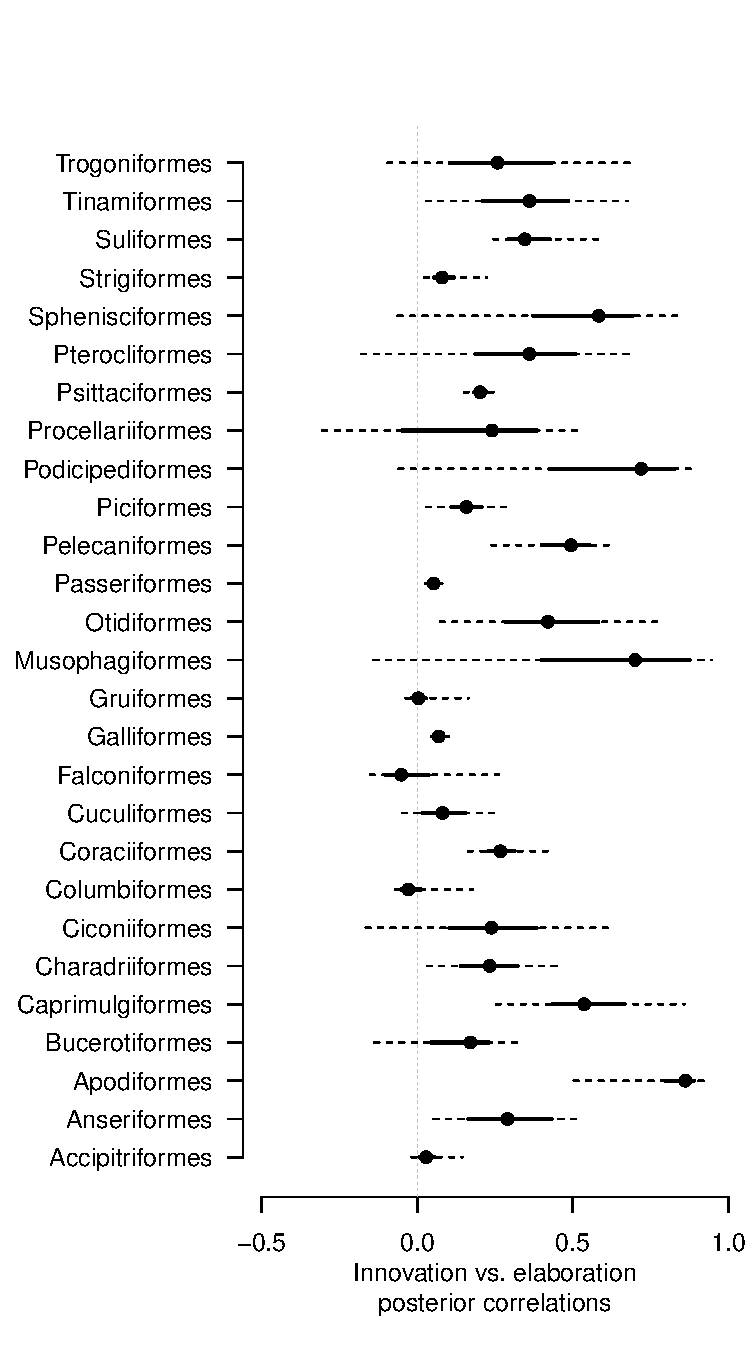
\includegraphics[width=0.5\textwidth]{Figures/correlations_fable_orders.pdf}
\caption{Posterior correlations between $elaboration_{species}$ and $innovation_{species}$ for each super-order. The dots, thick lines and dashed lines represent respectively the median, 50\% confidence interval (CI) and 95\% CI scores. 14 out of 27 of the orders have a clear posterior correlation between $elaboration_{species}$ and $innovation_{species}$ (i.e. 95\% CI does not overlap with 0), nine have a somewhat positive posterior correlation (i.e. 50\% CI does not overlap with 0) and four have no clear posterior correlation. Note that no order has a clear negative posterior correlation. This trend suggests that there is no tradeoff between $elaboration_{species}$ and $innovation_{species}$ and that both can be common routes for beak shape evolution at the macroevolutionary scale.
}
\label{fable_correlations}
\end{figure}
\bigskip

\newpage

\textcolor{blue}{Overall, I think the Results are written in a slightly disorganised and convoluted way (e.g., lines 91-94) and that could be easily improved.}

We have re-written the results, and reframed the manuscript to only focus on $elaboration_{species}$ and $innovation_{species}$ projected on their order’s major axis. e.g. lines 158-162:

\noindent{We found typically higher values of $elaboration_{species}$ than $innovation_{species}$ (Fig. \ref{Fig:phylogeny}) %@L_rephrase_wefound
and strong clustering of both $elaboration_{species}$ and $innovation_{species}$ (median $elaboration_{species}$ for all orders = 0.114, 95\%CI = 0.004-0.485;  $elaboration_{species}$ Pagel's $\lambda$ = 0.888; median $innovation_{species}$ for all orders = 0.071, 95\%CI = 0.018-0.224); $innovation_{species}$ Pagel's $\lambda$ = 0.848).%@L_ei_species_values. }


\textcolor{blue}{Figures:
I think the figures can be significantly improved. I personally feel it would be a pity that this important study will go unnoticed because the figures are less intuitive or aesthetic than they could be, so, I suggest that the authors could put a bit more emphasis on trying to make them easier to read.}

We have improved and modified our figures as suggested below, so hopefully they are now more intuitive.

\textcolor{blue}{Figure 1:Considering colours carry meaning in this figure I suggest removing clade colours and using alternate shades of grey or of one single hue as per Cooney, Bright et al., 2017, for instance. Some silhouettes for each major clade could better guide the readership.
I also suggest using one palette for innovation and another one for elaboration. These palettes would ideally go from grey for low values to a single hue for high values (e.g., orange for innovation; blue for elaboration).}

We tried adding silhouettes to the former figure 1 (now figure 2; circular phylogeny) however, due to the imbalance in clade sizes, the silhouettes are either mostly clumped in one portion ofthe tree due to the dominance of the passerines which looks unpleasant, or if they are spread evenly they are not next to the correct clade which is misleading. Therefore we have chosen to omit silhouettes but have overall simplified the figure. We do this by removing the innovation and elaboration scores for the whole phylogeny and the super-orders and standardised innovation and elaboration colour gradients as suggested (this was a really good suggestion, thanks). We have now changed the colour coding throughout the manuscript using orange for elaboration and blue for innovation. When showing gradients of either elaboration and innovation we are now using a gradient from grey (0) to orange/blue (highest value of elaboration/innovation) as suggested.

\textcolor{blue}{Some typos in the caption. Fix please. There is some text that is not very clearly written – check please.}

Fixed.

\textcolor{blue}{‘Blue and yellow colours on the branches of the phylogeny highlight species with relatively low distances to the global centroid of trait space whereas orange to red colours indicate high distance from the centroid’. In your figure the branch colours go from blue to yellow.}

Fixed.


\textcolor{blue}{Finally, I really do not understand the left boxplot inset.}

We have removed these boxplots altogether since we now only focus on the distribution of elaboration and innovation at the order level for the main text.

\begin{figure}[!htbp]
\centering
   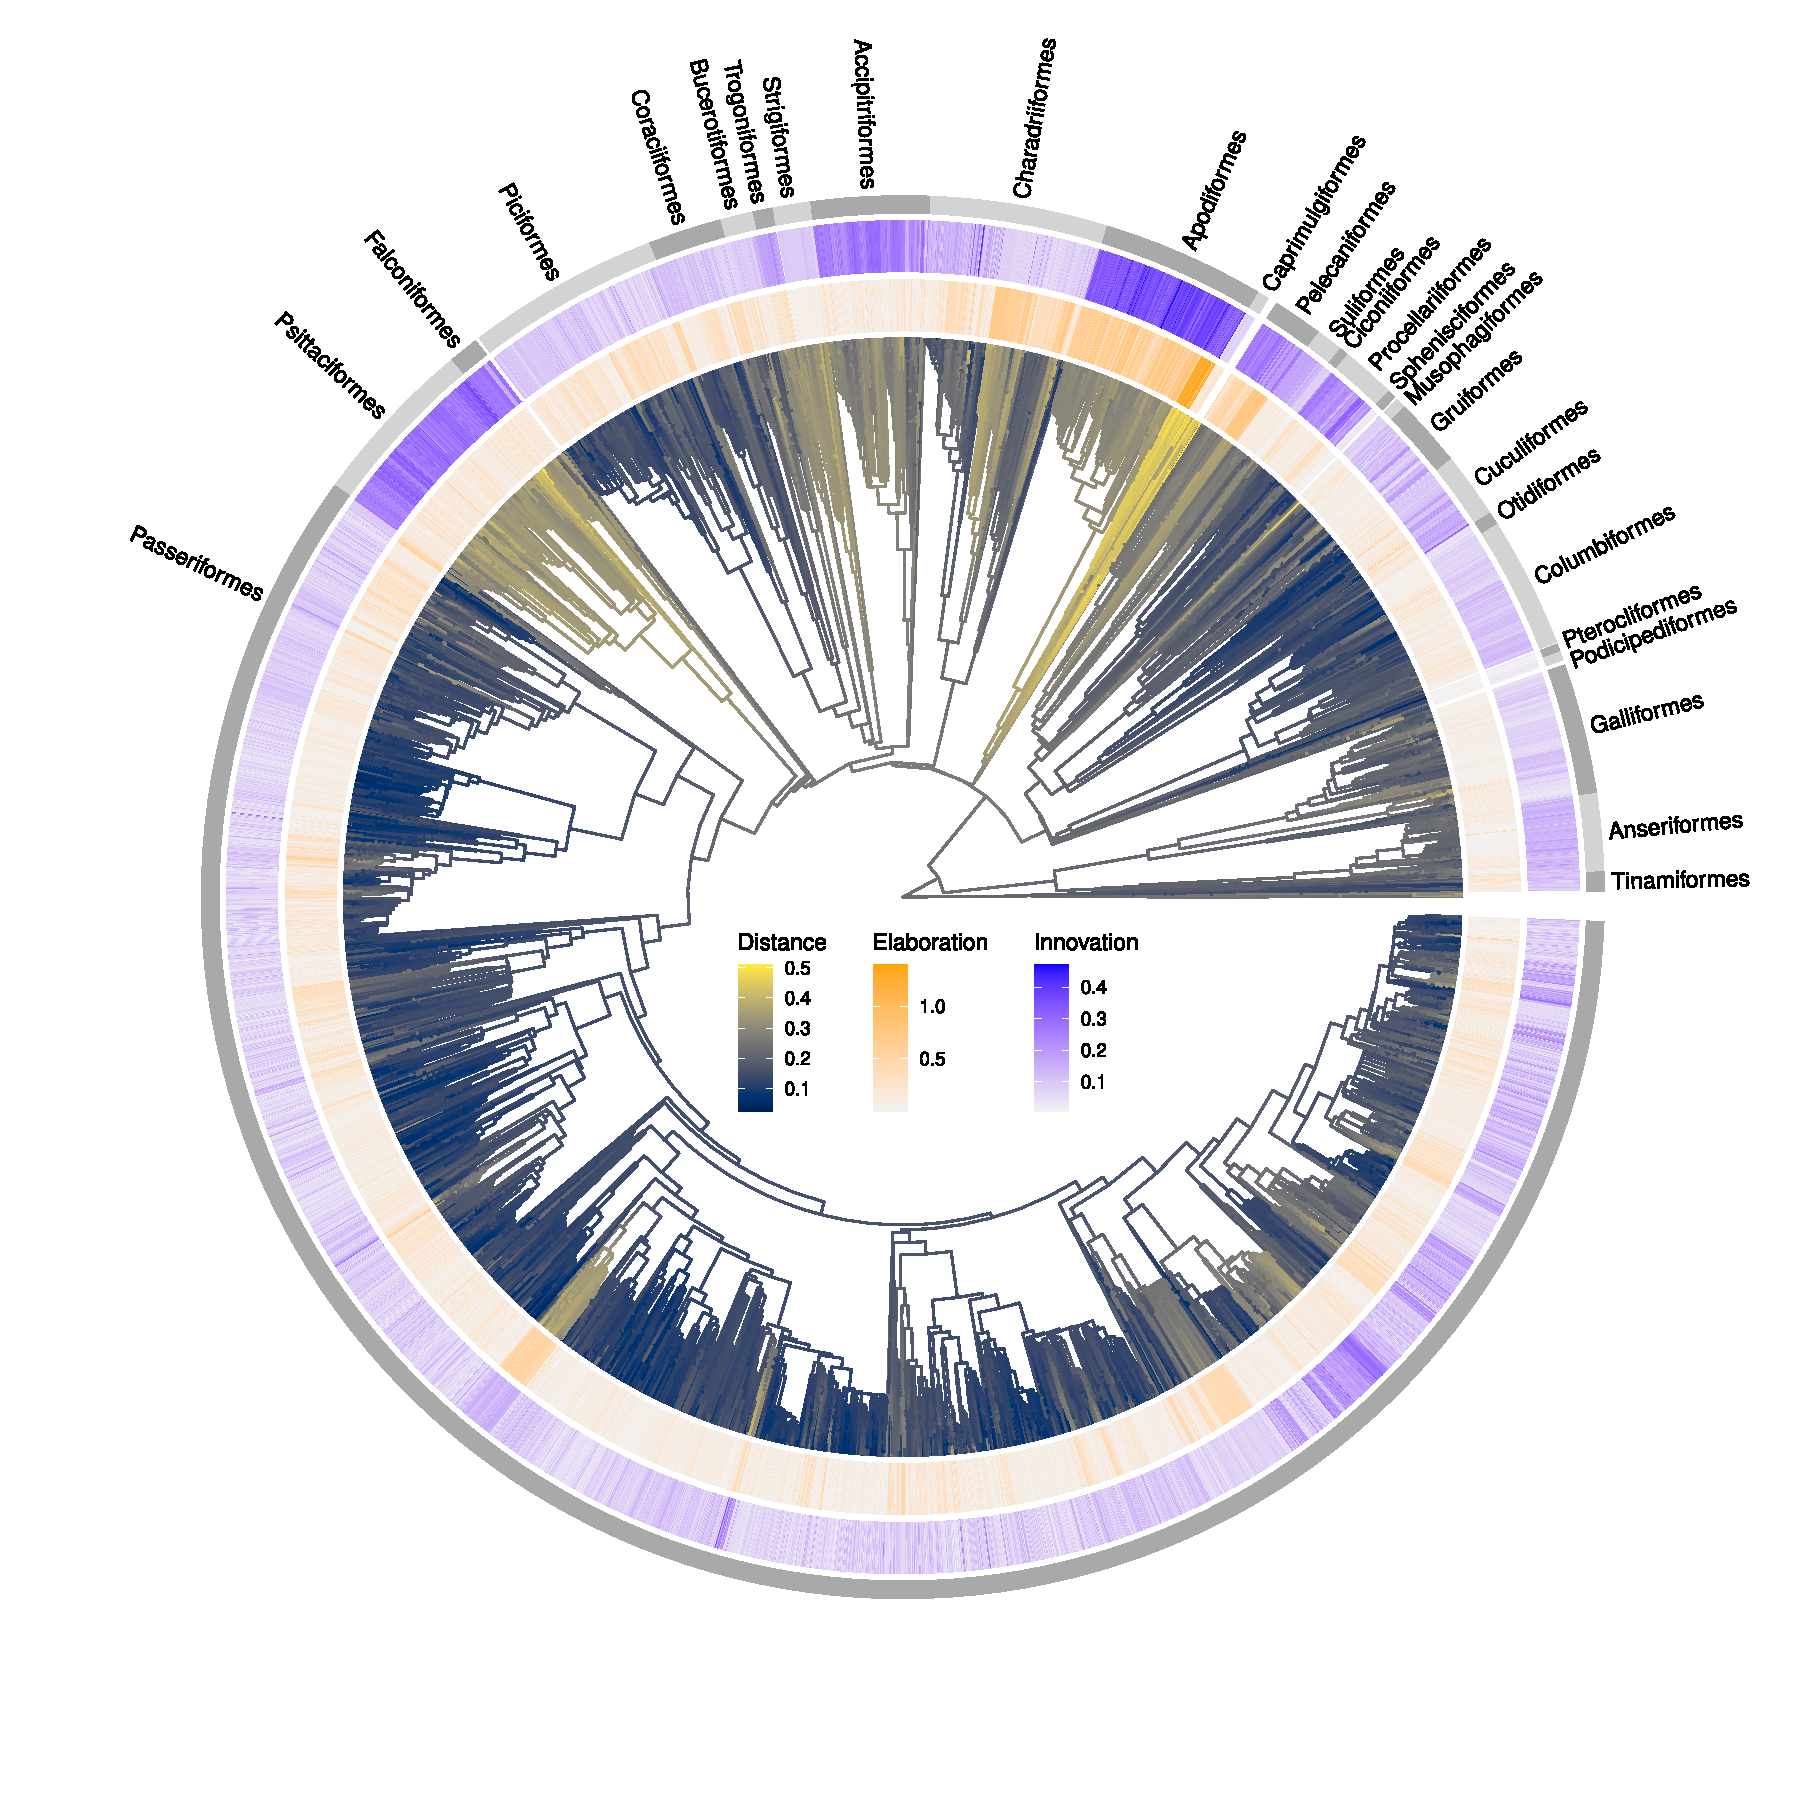
\includegraphics[width=0.8\textwidth]{Figures/InnovElabTree_main_text_revision.pdf}
\caption{Avian phylogeny (n = 8748 species) showing Euclidean distance of species to the centroid of beak space (branches, cividis scale), and distributions of species beak shape $elaboration_{species}$ (inner circle, orange scale), and $innovation_{species}$ (outer circle, blue scale).
Elaboration and innovation scores represent comparisons of species at the order level.
Additional comparisons to super-orders and at the class-wide phylogenetic level are shown in Fig. \ref{Fig:phylogeny_supplement} and for family and super-family comparisons of the order Passeriformes in Fig. \ref{fig_phylogeny_passeriformes}.
}
\label{Fig:phylogeny}
\end{figure}
\bigskip

\textcolor{blue}{Figure 2: I think you could use another colour that shows better contrast among each other perhaps using a palette which is not the default from ggplot. Also please label elaboration and innovation in the boxplots by each clades plot.}

The colour palette used here is not from ggplot (although we agree it looks very similar) and was chosen to offer the maximum contrast gradient among lineages. However, we agree that it is difficult to discern the different colours (it’s hard to find a palette for 35 nested variables!), so we have removed the colours from this plot. We have also completely reworked figure 2 (now figure 3) so it is now presented in a phylogenetic format with the super-orders overlapping the orders. We have also standardised the colours for elaboration (orange) and innovation (blue) as suggested in the comment about figure 1 above.

\newpage

\begin{figure}[!htbp]
\centering
   \includegraphics[width=0.6\textwidth]{Figures/figure_phylo_spiro_dark.pdf}
\caption{\scriptsize{$Elaboration_{clade}$ and $innovation_{clade}$ at the megaevolutionary scale for each order and super-order in the bird phylogeny.
The black and gray ellipses are the scaled average evolutionary rate matrices from the pGLMM models for respectively the clades (black) and the class-wide phylogeny (gray).
The ellipses are centered on the position of the clade in the shapespace.
The associated black bar plots represent the variance on each of the eight dimensions in the shapespace with the top gray bar plot representing the variance on each of the eight dimensions for the class-wide phylogeny.
The orange and blue distributions represent respectively the distribution of the $elaboration_{clade}$ (orange) and the $innovation_{clade}$ (blue) scores for each clade and the dots are the median $elaboration_{clade}$ or $innovation_{clade}$ and the solid and the dashed lines representing the 50\% and the 95\% confidence intervales of the distribution of the scores across the 4000 posterior samples.
The ticks on the y-axis always represent five arbitrary units of elaboration and innovation.
An alternative visualization of the same information is available in the supplementary materials in Fig. \ref{Fig:ellipses_rainbow} along with a companion plot showing further nested structure within the Passeriformes in Fig. \ref{fig_ellipses_passeriformes}.}
}
\label{Fig:ellipses}
\end{figure}

\newpage

\textcolor{blue}{Figure S5 caption: ‘The distribution of innovation and elaboration scores comes from the projection of the 4000 pairs of posterior VCVs.’ It would be good to briefly state where these 4k pairs are.}

We have now integrated Figure S5 into the main text (as figure 1) and have completely rewritten the caption (including the precision of what these pairs are). See comment above referring to now figure 1:


\noindent\textit{Relationships between key figures in the main text.
A) represents the two first principal components (PCs) of the eight dimensional trait space with all bird beak shapes represented as gray circles and the Tinamiformes as red circles.
The gray ellipse represents the overall phylogenetic major axis of beak variation in birds.
Species aligned or away from this axis are respectively elaborators or innovators relative to the class Aves.
The red ellipse and axis represents the phylogenetic major axis of beak variation in Tinamiformes only.
Species aligned or away from this axis are respectively elaborators and innovators relative to the Tinamiformes order.
B) In Figure 2, we measured elaboration and innovation at the macroevolutionary scale , i.e. the position of each species in terms of $elaboration_{species}$ and $innovation_{species}$ relative to their order's phylogenetic major axis of beak variation.
A species $elaboration_{species}$ score is the species projection onto their order's phylogenetic major axis of beak variation(i. e. their position on that axis) whereas their $innovation_{species}$ score is their rejection from it (i.e. their distance away from that axis).
The colours on the tips of the phylogeny correspond to the median $elaboration_{species}$ (orange gradient) and $innovation_{species}$ (blue gradient).
C) Figure 4, we measured elaboration and innovation at the megaevolutionary scale, i.e. $elaboration_{clade}$ and $innovation_{clade}$.
The ellipses are scaled and centered and represent the clade's phylogenetic major axis of beak variation relative to the overall phylogenetic major axis of beak variation with the relative length of the ellipse on each dimension represented on the barplots as variance on each dimension.
A clade's $elaboration_{clade}$ and $innovation_{clade}$ scores are measured by projecting the clade's phylogenetic major axis of beak variation onto the overall phylogenetic major axis of beak variation and measuring the projection (elaboration) and rejection (innovation) from this axis as described above.
The distribution elaboration and innovation scores are taken from the projection of the 4000 pairs of evolutionary rate matrices with each pair being the focal level, e.g. order,and the parent level, e.g. the whole bird phylogeny.}



\bibliographystyle{naturemag}
\bibliography{references}

\end{document}
